\chapter{Partition sums of repetitive DNA}
\label{app:DNA_partitionsums}
The analytic results obtained in the publications reprinted in \SEC{DNA_sliding} rely to a great extent
on the calculation of the partition sum of repetitive double stranded DNA molecules. How this partition sum
is calculated was discussed only briefly and I want to present the important steps in greater detail here.
When the two strands have a repetitive and complementary sequence, the approximation that
only native base pairs form is no longer justified. To the contrary, each repeat unit from one strand 
can bind to every repeat unit of the other strand. The configurations that contribute to the partition sum  
are therefore much more numerous and the calculation is considerably harder.
The only assumption that can be reasonably made, is that base pairs do not cross, \emph{i.e.}~that 
the molecule can be depicted as a sequence of denatured loops and double stranded helices. However, the
loops can now have a different number of bases on the two strands. 

Every allowed configuration can be broken into essentially two different parts: the four open ends
and the central part that is bounded by base pairs as illustrated in \FIG{partition}. 
\begin{figure}
\centering
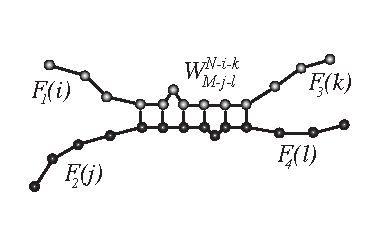
\includegraphics[width=\halffigure]{\FIGPATH/Figures_Partitionsum/partition}
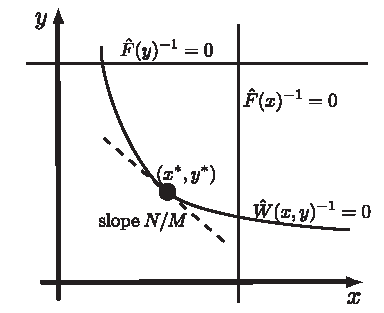
\includegraphics[width=\halffigure]{\FIGPATH/Figures_Partitionsum/poles}
\caption[Calculating the partition sum.]{\label{fig:partition}Left: Every base-pairing configuration can be described by the length of the single stranded ends 1 to 4 and the part bounded by base pairs.
Right: A sketch of the singularities of $\Fh(x)$, $\Fh(y)$ and $\Wh(x,y)$ in the positive quarter plane
of real $x$ and $y$. }
\end{figure}
The partition sum of the molecule with $N$ 
repeat units on one and $M$ repeat units on the other strand is thus given by
\begin{equation}
\label{eq:completeZ}
  Z(N,M)=\sum_{i,j,k,l=0}^{i+k< N, j+l< M}F_1(i)F_2(j)F_3(k)F_4(l)W_{M-j-l}^{N-i-k},
\end{equation}
where $F_i(n)$ are the statistical weights of the single stranded ends of length $n$ and $W_s^{r}$ is the sum of all possible configuration of a double stranded part with $r$ bases on one and $s$ bases on the other strand.
Similarly to the case where only native base pairs are allowed (see \SEC{DNA_melting}), $W_s^{r}$ can 
be calculated from the recursion relation
\begin{equation}
\label{eq:recursion}
  W_{s+1}^{r+1}=q_{s+1}^{r+1}W_{s}^r+q_{s+1}^{r+1}\sum_{k+m>1}^{k<r,m<s} \El(k,m)W_{s-m}^{r-k},
\end{equation}
where $q_{s}^{r}$ is the Boltzmann factor of the binding energy of base $r$ and base $s$ and $\El(k,m)$ is the cost 
of having a loop with $k$ bases on one and $m$ bases on the other strand. The first term of the
recursion relation accounts for all configuration where the base pair $(r+1,s+1)$ is added to 
any configuration in $W_{s}^r$, whereas the second term includes all configuration where the
base pair $(r+1,s+1)$ followed by a loop of size $(k,m)$ is added to any configuration in $W_{s-m}^{r-k}$.
One easily convinces oneself, that this recursion indeed generates all allowed configurations.

This recursion relation can be solved numerically for arbitrary sequences in $\mathcal{O}(N^{2}M^{2})$
operations \cite{Garel_Biopolymers_04, Bundschuh_PRE_02}. 
An analytical solution can be obtained, if the sequence is homogenous, that is  $q_{s}^{r}=q$,
and if $\El(k,m)$ is sufficiently well behaved. Note that every repetitive sequence is essentially homogeneous
since each repeat unit can be treated a single base which only binds to its native binding partner.
Again, the recursion relation can be solved by $z$-transformation, but this time different fugacities $x$ and $y$ 
for the two strands are needed since they can be of different length and are not necessarily in register. 
To this end, we multiply both sides by $x^{r}y^{s}$ and sum over $r$ and $s$ to obtain
\begin{equation}
\label{eq:recursion}
  \frac{\Wh(x,y)-xyW_1^{1}}{xy}=q\Wh(x,y)+q\Elh(x,y)\Wh(x,y),
\end{equation}
where $\Wh(x,y)=\sum_{r,s=1}^{\infty} W_s^{r}x^{r}y^{s}$, $\Elh(x,y)=\sum_{r,s=1}^{\infty} \El(r,s)x^{r}y^{s}$ and
$W_1^{i}=W_i^{1}=0$ for all $i>1$. This is readily solved for $\Wh(x,y)$, yielding
\begin{equation}
\label{eq:What}
 \Wh(x,y) = \frac{W_1^{1}}{\frac{1}{xy}-q-q\Elh(x,y)},
\end{equation}
The $z$-transform of the partition sum in \EQ{completeZ} is computed similarly and given by 
\begin{equation}
\label{eq:completeZ}
  \Zh(x,y)=\Fh_1(x)\Fh_2(y)\Fh_3(x)\Fh_4(y)\Wh(x,y),
\end{equation}
where $\Fh_i(z)$ is the one variable $z$-transform of the single stranded ends. 

The $z$-transformations in the base indices on both strands are equivalent to changing from a statistical 
ensemble with constant particle numbers to a grand ensemble, where the particle number is determined
by the fugacities of a particle reservoir. The grand partition sum is a power series in $x^{N}y^{M}$ with 
coefficients $Z(N,M)$. Therefore $Z(N,M)$ can in principle be obtained from $\Zh(x,y)$ by double contour integration
\begin{equation}
\label{eq:contour_int}
   Z(N,M)=-\frac{1}{4\pi^{2}}\oint\oint dxdy\;\frac{\Zh(x,y)}{x^{N+1}y^{M+1}}.
\end{equation}
In many cases, one of the integrals can be calculated by suitable deformation of the integration contour, but the
remaining integral is usually infeasible. Nevertheless, a great deal of information can be obtained from the 
function $\Zh(x,y)$, at least in the thermodynamic limit, which for linear molecules corresponds to the 
limit of long strands \cite{Tamm_PRE_07}. In this limit relative strand length fluctuations vanish and the grand ensemble is equivalent to the fixed length ensemble. The expected numbers of particles on both strands are given by 
\begin{equation}
\label{eq:mean_length}
\begin{split}
  \langle N \rangle= x\frac{\partial \ln\Zh(x,y)}{\partial x}\quad \mathrm{and}\quad
   \langle M \rangle= y\frac{\partial \ln\Zh(x,y)}{\partial y},
\end{split}
\end{equation}
and for $\langle N \rangle$ or $\langle M \rangle$ to become arbitrarily large, $\Zh(x,y)$ has to diverge. 
The thermodynamic limit
thus confines the set of possible fugacities to the singularities of $\Zh(x,y)$, which in general 
form a one dimensional, possibly multiply branched, set (cf.~right part of \FIG{partition}). 
To fix the fugacities completely, we need an additional condition. 
This is given by the requirement, that the ratio of the two strand length remains constant
as the thermodynamic limit is approaches. Otherwise, the intensive properties of the system 
are not preserved. We thus have to choose the fugacities $(\xf, \yf)$ such that
\begin{eqnarray}
\label{eq:partsum_divergence}
 \nonumber
  &\lim_{x,y\rightarrow \xf,\yf}\langle N \rangle= \infty \qquad \mathrm{and}\qquad \lim_{x,y\rightarrow \xf,\yf}\langle M \rangle= \infty\\
&\lim_{x,y\rightarrow \xf,\yf}\frac{\langle N \rangle}{\langle M \rangle}=c. 
\end{eqnarray}
Since the free energy of the DNA molecule should be extensive, the partition sum for long strands of 
length $N$ and $cN$ is of the form $Z(N, cN )= \gamma^{N}$.
From the definition $\Zh(x,y)=\sum_{N,M=1}^{\infty} Z(N,M)x^{N}y^{M}$ and the fact that only 
configurations with $M\approx Nc$ contribute, we have 
$\Zh(x,y)\sim(1-\gamma^{N}x^{N}y^{cM})^{-1}$. Hence, the singularities of $\Zh(x,y)$ lie on the curve 
$\xf\yf^{c}=\gamma^{-1}$. The limit of infinite strand length is approached from below $|xy^{c}|<\gamma^{-1}$. 
Within this approximation, which essentially is a saddle point approximation, the free energy of a 
molecule out of strands of length $N$ and $M$ is given by 
\begin{equation}
\label{eq:free_energy}
   F(N,M)=-\kT\ln Z(N,M) = N \ln \xf + M \ln \yf,
\end{equation}
where the free energies per base $\ln \xf$ and $\ln \yf$ are determined by \EQ{partsum_divergence} and 
\EQ{mean_length}. Alternatively, one can perform the inverse transformation in one variable and thereby 
fix one strand length and then determine the remaining fugacity such that the expected length of the 
other strands matches the desired value. We will now apply this formalism to concrete problems of
repetitive DNA under shear force and thermal denaturation of DNA. 
A more detailed description of this derivation is given in \REF{Tamm_PRE_07}.
 
\section{Thermal denaturation of repetitive DNA}
To describe the melting transition of repetitive DNA, we have to specify the Boltzmann factor associated with
the binding of one repeat unit and the statistical weights of loops and single stranded ends. 
The statistical weights of loops and free ends are dominated by the entropy of the different 
configurations available to the flexible polymer, as already discussed in \SEC{DNA_melting}. 
The statistical weights of free single stranded ends of length $n$ and of loops with $n$ and $m$
on the two strands are given by
\begin{equation}
F(n)=\frac{s^n}{n^{\bar{c}}} \qquad \mathrm{and} \qquad \El(n,m)=g^{2}\frac{s^{n+m}}{(n+m)^c},
\end{equation}
where the exponents $\bar{c}$ and $c$ describe the excluded volume effects of an open end and 
a closed loop. While $\bar{c}$ is irrelevant for the melting transition, $c$ is pivotal and its value is assumed 
to lie in the range $1.8\ldots2.15$ \cite{Kafri_PRL_00} (cf.~\SEC{DNA_melting}). 
The $z$ transformations of the weights are given by
\begin{equation}
\Fh(x)=\Phi_{\bar{c}}(xs) \qquad \mathrm{and} \qquad \Elh(x,y)=g^{2}\frac{x\Phi_c(xs)-y\Phi_c(ys)}{x-y}.
\end{equation}
The factor $g^{2}$ accounts for a finite energy penalty to initiate a loop. The function $\Phi_c(z)$
is the polylogarithm, which is analytic everywhere in the complex plane, except on the interval
$[1,\infty[$ of the real axis. 

Inserting $\Fh(x)$ and $\Elh(x,y)$ into equation \EQ{completeZ} yields the grand canonical 
partition sum two homogeneous DNA strands. As described above, the asymptotic behavior of 
the two strands is governed by the singularity of $\Zh(x,y)$ which is closest to the origin, subject to the
constraint that the ratio of the two strand length is fixed. 
Depending on whether this singularity is the branch-cut induced by the polylogarithm 
or an isolated singularity of  $\Wh(x,y)$, the two strands are denatured or bound to each other. 
The phase behavior of such systems is discussed in \SEC{intermediate_phase}.

\section{Pulling on repetitive DNA}
When exerting a shear force to the DNA, we have to distinguish between ends where the 
force is applied to and the unstretched ends. From now on, we model the ssDNA by the freely jointed 
chain (FJC) model, neglecting self-avoidance. Furthermore, we give all energies relative 
to unconstrained single strand. Consequently, for unstretched ends we have $F_{2}(n)=1$
 irrespective of the length $n$. The transformed $\Fh_{2}(x)$ is given by $(1-x)^{{-1}}$. 
 The free energy of the DNA molecule in the external force field is given by the product
 of an effective length $L$ and the magnitude of the force. This effective length can be calculated
 separately for the single stranded ends and the double stranded region in between.  
The free energy of a segment of a FJC polymer with Kuhn length $l_k$ under a tension 
 $f$ is given by the integral over all orientations of a segment
\begin{equation}
\frac{1}{2}\int e^{-\frac{fl_k\cos \theta}{\kT}}\sin \theta d\theta=\frac{\kT}{fl_k}\sinh\left(\frac{fl_k}{\kT}\right).
\end{equation}
The free energy per monomer of length $\lss$ is thus given by 
$f\cdot\tss=\frac{\lss}{l_k}\ln\left(\frac{\kT}{fl_k}\sinh\left(\frac{fl_k}{\kT}\right)\right)$, 
where $\tss$ is an effective length. The contribution of stretched ssDNA of length $n$ is 
therefore $F_{1}(n,f)=e^{n \tss f}=\ebs^n$ and its $z$-transform reads $\Fh_{1}(x,f)=(1-x\ebs)^{-1}$.
dsDNA is sufficiently stiff and long, such that we can assume that its completely aligned, yielding 
a free energy per base pair $f\cdot\lds$.  Together with the binding free energy the statistical weight
of a base pair is given by $q=e^{f\lds+\eps}=\ebd q_0$. 
The statistical weights of loops within the sequence is a bit more subtle to calculate. We assume, 
that the projected length of a loop is given by the length the shorter arm would have when in a double
helix. As loop cost function, we use  $\El(n,m,f)=g^{2}e^{\lds\min(n,m)f}=g^{2}\ebd^{\min(n,m)}$, where $g^{2}$ accounts for loop initiation and the exponential for the stretching energy. 
The two variable $z$-transformation of this quantity is a bit laborious and yields
\begin{equation}
\Elh(x,y,f)=\frac{g^2}{1-\ebd xy}\left(\frac{x}{1-x}+\frac{y}{1-y}+\ebd\right)
\end{equation}
Inserting the different functions for loop cost and single strand contributions in \EQ{completeZ}
yields the grand canonical partition sum for sheared DNA. The single strand factors have obvious
singularities at $x=1$, $y=1$, $x=\ebs^{-1}$ and $y=\eps^{-1}$, corresponding to no stable binding 
 and completely stretched single strand, respectively. At low forces, however, $\Wh(x,y)$ has
an additional singularity at $(\xf, \yf)$ corresponding to a state where the two strands bind with maximal 
overlap. The transition from this bound state the stretched state occurs when $(\xf,\yf) = (\ebs^{-1}, \ebs^{-1})$.
In the limit of high loop cost the contribution $\Elh(x,y,f)$ in the denominator can be neglected and 
it is easily seen that the singularity is found at $\xf\yf=\ebd q_0$. The transition to the open state
occurs at $\xf\yf=\ebs^{-2}=\ebd q_0$, which is yields $\fc=\frac{\eps}{2\tss-\lds}$. At finite loop
cost the double stranded region is stabilized by the combinatorial entropy of the different double stranded
conformations. Typically, this contribution is small.


\subsection{Determining loop densities.}
In \SEC{DNA_sliding}, it was argued that the sliding velocities can be calculated from the 
pseudo-equilibrium loop densities, which in turn can be calculated from the proper equilibrium 
properties of a suitably chosen system. This system cannot be a double
strand with a shear force applied, since at equilibrium in the supercritical regime, there is no double stranded
region and no loop density can be defined. The argument leading to the pseudo-equilibirium density 
was, that the two strands move slowly relative to each other, such that the densities at the ends 
equilibrate. We now idealize this assumption, by attaching both strands to a wall at one end, and apply
a force to the longer strand at the other end, at illustrated in \FIG{loop_densities}.
\begin{figure}
\centering
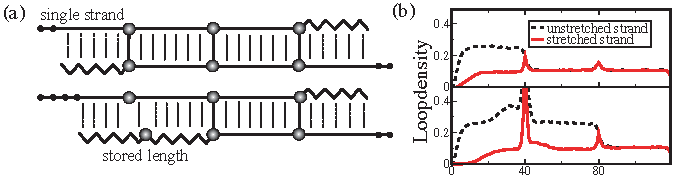
\includegraphics[width=\smallfigure]{\FIGPATH/Figures_Partitionsum/loopdensities}
\caption[Calculating loop densities.]{\label{fig:loop_densities} Using a double strand attached to a wall, we can 
calculate the loop densities on the stretched and unstretched strands, even for $f>\fc$.}
\end{figure}
The partition sum of this system is given by 
\begin{equation}
\label{eq:Z_fdenat}
  \Zh(x,y)=\Fh_s(x)\Fh_u(y)\Wh(x,y),
\end{equation}
where the stretched single strand contributes $\Fh_s(x)=(1-x\ebs^{{-1}})$, the unstretched single strand
$\Fh_u(y)=(1-y)^{-1}$ and $\Wh(x,y)$ is the same as above. Given the complete partition sum, we can now
calculate the average number of base pairs via
\begin{equation}
	\langle N_{bp}\rangle=\frac{\partial \ln \Zh(x,y)}{\partial \ln q}.
\end{equation}
Furthermore, we can calculate the number of nucleotides on the upper and lower strand inside the 
double helical region by 
\begin{equation}
	\langle N_{u}\rangle=\frac{\partial \ln \Wh(x,y)}{\partial \ln x} \qquad \mathrm{and} \qquad
	\langle N_{l}\rangle=\frac{\partial \ln \Wh(x,y)}{\partial \ln y}.
\end{equation}
Similarily, we can calculate the average number of loops inside the double helical region by differentiating
$\ln \Zh(x,y)$ with respect to $2\ln g$. From these quantities the loop densities, the stored length and 
the mean loop size are readily calculated. 



